% BACKGROUND & RELATED WORK
%
% !TEX root = ../thesis-main.tex
%
\chapter{Background and related work}
\label{chap:background}

%\cleanchapterquote{You can’t do better design with a computer, but you can speed up your work enormously.}{Wim Crouwel}{(Graphic designer and typographer)}




\section{Computer-Assisted Pronunciation Training} %TODO Teaching,Training?
\label{sec:bkgd:capt}

	\citep{Eskenazi2009,Delmonte2011,Witt2012}

	\subsection{Pronunciation in foreign language education}
	\label{sec:capt:l2ed}
	
	The difficulties posed by including pronunciation in the foreign language classroom curriculum will be discussed in this section, leading to the conclusion that CAPT can help make pronunciation training more accessible by overcoming some of these difficulties (e.g. teacher-to-student ratio). Relevant findings from a variety of works on pronunciation teaching in the classroom will be presented \citep{Derwing2005,Dlaska2013,Hirschfeld2007,Mehlhorn2005}.

	\subsection{Computer-based and intelligent tutoring systems?} 
	\label{sec:capt:its}
	%TODO is this section necessary?
	
	This section would serve as a domain-independent overview of CBT and ITS, and the advantages such systems can bring when deployed in schools or used individually.
	
	\subsection{Prosody in existing CAPT systems}
	\label{sec:capt:systems}
	
	This section will describe a selection of related CAPT systems and tools, and how these tools have analyzed and offered feedback on speech prosody.
	
	Both the diagnosis and feedback modules of the CAPT tool will build to a great extent on work conducted by the speech group at LORIA in Nancy \citep{Bonneau2011,Fohr1996,Fohr2012,Mesbahi2011,Orosanu2012}. The Jsnoori/WinSnoori software \citep{Parole2013} %TODO properly cite Jsnoori/WinSnoori?
which this group has developed will be instrumental in the construction of the CAPT tool. 
	
	This work will also draw from research conducted at Carnegie Mellon University in Pittsburgh, particularly in the context of the FLUENCY pronunciation training system \cite{Eskenazi1998,Probst2002} and the LISTEN project and its Reading Tutor \citep{Duong2011,Mostow2012,Mostow1999,Sitaram2011,Weber2010}. The latter may not strictly fall into the category of CAPT systems, but as it analyzes the prosody of children's read speech to measure reading fluency, and offers feedback on this prosody, it is nevertheless very relevant to this thesis.
	
	Other systems mentioned by \textcite{Eskenazi2009,Delmonte2011,Witt2012} may also be briefly described, including tools developed at KTH \citep{Hincks2002,Hincks2009} to teach English prosody.
	
	
% Alternative organization:
 \section{Lexical stress}
 \label{sec:bkgd:stress}
		%TODO check this section for inaccuracies
			Lexical stress is the phenomenon of how syllables are accentuated within a word  \citep{Cutler2005}. This relates not to the segmental characteristics of a syllable, i.e. the speech sounds it contains, but rather to its (relative) suprasegmental properties, namely: %TODO need citation here?
			\begin{itemize}
			\item duration, which equates on the perceptual level to timing;
			\item fundamental frequency (F0), which corresponds to perceived pitch; and
			\item intensity (energy or amplitude), which perceptually equates to loudness.
			\end{itemize}

%TODO more text here? or move text from German vs French section here?
		
		%\subsection{German vs. French}
		%\label{sec:stress:GvF}
		
					As \textcite{Cutler2005} points out, different languages make use of this suprasegmental information in different ways. 
			In what are termed free- or variable-stress languages, such as German, Spanish, and English, it is not always possible to predict which syllable in a word will carry the stress, and therefore knowing a word requires, in part, knowing its stress pattern. This allows stress to serve a contrastive function in these languages, such that two words may share exactly the same sequence of phones and nevertheless be distinguished exclusively by their stress pattern, as is the case with X and Y in German. %TODO example of minimal pair
Because stress carries meaning thus, native speakers of such languages are sensitive to stress patterns, and readily able to perceive differences in stress. %TODO wording?

			However, in the so-called fixed-stress languages, stress is completely predictable, as it always falls on a certain position in the word; in Czech and Hungarian, for example, stress always falls on the word-initial syllable. Therefore, lexical stress may not be as crucial to the knowledge of a word in these languages as in the free-stress languages. Furthermore, although lexical stress is realized in these languages, the distinction between stressed and unstressed syllables may be weaker than in free-stress languages. French has often been placed into this category of fixed-stress languages, although it may be more properly considered a language without lexical stress, insofar as there is no systematic way in which speakers distinguish a certain syllable from others in the word, aside from the fact that French exhibits phrasal accent, i.e. lengthening of the final syllable in each prosodic group or phrase \citep{Dupoux2008}. %TODO other references?			
			
		Therefore, native speakers of French may lack the sensitivity to stress patterns possessed by native speakers of German. Indeed, this has been borne out by research by \citeauthor{Dupoux2008} \citep{Peperkamp2002,Dupoux2001,Dupoux2008}, which demonstrated that native French speakers were ``deaf'' to differences in stress patterns, such that they have great difficulty discriminating between Spanish words which contrast only at the level of stress. This difficulty should therefore also exist for French speakers when they are presented with German words in which the stress pattern is crucial to the word's meaning, as in the minimal pair above.
		
%		\subsection{Lexical stress in foreign language teaching?}
%		\label{sec:stress:l2ed}
%		
%		This section may be merged into \cref{sec:capt:l2ed} above.
%		
%		\citep{Hirschfeld2007}
		
		
 \section{Targeting lexical stress errors in CAPT}
 \label{sec:bkgd:targeting}
 	Learners of a foreign language typically make a wide variety of pronunciation errors, at both the segmental level (e.g. errors in producing certain individual phones of the target language) and the prosodic level (e.g. errors in the speaker's intonation contour or the duration of certain syllables or words). As it is not possible to address all of these in an automated system, one of the first aims of this work is to identify a single type of error which is well suited to being addressed via a CAPT system targeting French L1 learners of German as the L2. 
	
	To guide this selection, we may consider %TODO wording
a set of three criteria that such an error must meet. 
%As illustrated in \cref{fig:errors}, t %TODO replace reference after proposal
The best error to target with the CAPT system will fulfill all of these criteria, rather than only one or two of the three. 
First, the error must be produced with a some degree of frequency by French L1 speakers in their production of L2 German, as it would be a misuse of resources to design a system which addresses an error that is seldom made by learners. Secondly, the given error must have a significant impact on the perceived intelligibility of the learner's speech; as the ultimate goal of the system is to help learners communicate more effectively in the L2, an error which is commonly made but nevertheless does not impede understanding of the learner's L2 speech, and thus does not hinder communication in the L2, is not an ideal target. Finally, in order for the CAPT system to provide any meaningful diagnosis of and feedback on the error, it must lend itself to reasonably accurate and reliable  detection through automatic processing. 
	
%TODO replace figure after proposal
%		%\begin{center}
%		\begin{figure}[htb]
%			\centering
%			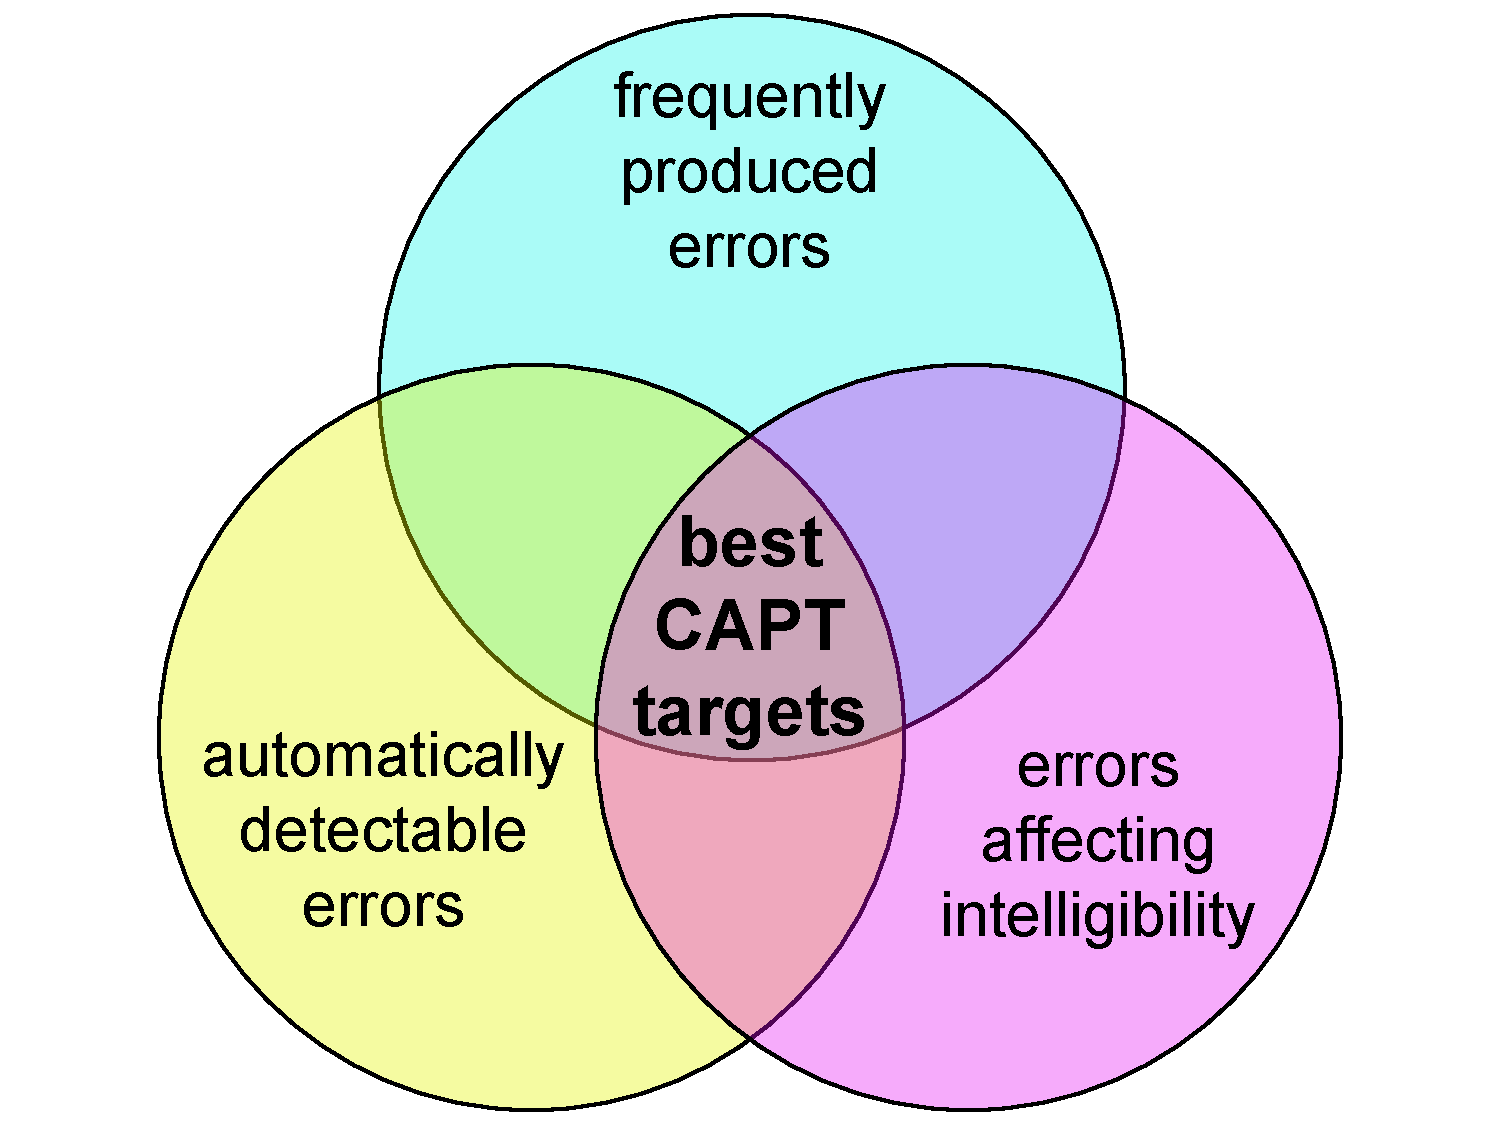
\includegraphics[width=.7\textwidth]{../img/error-venn}
%			\caption{Criteria for selecting errors to target in a CAPT system.}
%			\label{fig:errors}
%		\end{figure}
%		%\end{center}
	
	This thesis proposes that lexical stress errors are a strong candidate for treatment via CAPT, and will therefore be the focus of the prototype system which will be developed. The remainder of this section justifies the targeting of lexical stress errors by describing how this type of error fulfills the aforementioned criteria.
	 
	 %TODO take the below out?
	 %For example, vowel quality errors (e.g. an L1 French speaker producing a German /\textipa{@}/ as [\textipa{\oe}]) may occur frequently in the L2 speech and may be relatively easy to detect automatically, but may not have a great impact on the intelligibility of the L2 German speech. On the other hand, equally frequent vowel quantity errors (e.g. the L1 French speaker producing a German long /\textipa{e:}/ as [\textipa{e}]) may have a greater impact on intelligibility in some cases, but may be more difficult to reliably identify automatically.
	
%TODO remove
	%Analysis of the typical and expected errors described in \cref{sec:CAPT4FG:comparison} in terms of these criteria reveals that lexical stress errors are a strong candidate for treatment via CAPT, and will therefore be the focus of the prototype CAPT system described in this thesis. The remainder of this section justifies the selection of this type of error by describing how it fulfills the aforementioned criteria as well or better than any other error type.
	

%TODO replace
%		\subsection{Impact on intelligibility}
%		\label{sec:targeting:intelligibility}
		\citep{Warren2009}
		
		\citep{Magen1998}
		
		Stress errors may affect perception of segmental errors; errors in stressed syllables are more noticeable \citep{Cutler2005}
				
%TODO replace	
%		\subsection{Frequency of production}
%		\label{sec:targeting:frequency}
		\citep{Cutler2005}
		
		\citep{Peperkamp2002, Dupoux2001, Dupoux2008}
		
%TODO replace
%		\subsection{Feasibility of automatic detection}
%		\label{sec:targeting:autodetect}
		\citep{ISADEPT, Delmonte2011}
		
		\citep{Bonneau2011}
		
		\citep{Shahin2012a,Kim2011}
		
% \section or \subsection{Other related work on lexical stress in CAPT}

% Old section:
%\section{Towards CAPT for French learners of German}
%\label{sec:CAPT4FG}
	
% Alternative organization:
%	\subsection{Targeting errors in CAPT}
%	\subsection{Lexical stress in French and German}
%	\subsection{Targeting lexical stress errors}

% Old organization:
%	\subsection{Phonetic and phonological comparison}
%	\label{sec:CAPT4FG:comparison}
%		\subsubsection{Segments}
%		\subsubsection{Prosody}
%
%			\paragraph{Lexical stress}
%			
%		\subsubsection{Other factors}
%		
%	\subsection{Targeting lexical stress errors}
%	\label{sec:CAPT4FG:targeting}
%
%		\subsubsection{Frequency of production}
%		
%		\subsubsection{Impact on intelligibility}
%		
%		\subsubsection{Feasibility of automatic detection}
%		

%TODO replace
%\section{Summary}
%\label{sec:bkgd:summary}